\section{Electromagnetic Calorimeter}
\label{sec:ecal}
The electromagnetic calorimeter (ECAL) was designed with the specification of measuring the energy of particles that interact electromagnetically with a very high precision. 
The search for the Higgs boson in the channel $H\rightarrow\gamma\gamma$ was a driving factor in the design of the ECAL.
The ECAL is a hermetic, homogeneous detector constructed of scintillating lead tungstate (\ce{PbWO4}) crystals, 61200 in the barrel region, and 7324 in each of the endcaps.
Particles that interact electromagnetically, primarily electrons and photons, will cause electromagnetic showers in the ECAL material.
An electromagnetic shower is a process in which electrons and photons are created, via pair-production or bremsstrahlung respectively.
The ultimate conclusion of an electromagnetic shower is a collection of scintillation photons that are measured by photo multipliers which read out the signal of each crystal. %FIXME diodes?
The energy of the particle inducing the shower can be inferred from the number of photons that are collected.

To reliably measure the energy of an incident electron or photon, the total energy of the particle must be absorbed by the calorimeter, and thus a crystal must be capable of capturing the entire shower of a particle longitudinally.
The ability of the crystal to confine an electromagnetic shower is dependent on the depth of the crystal, the density of the crystal, and the radiation length of an electromagnetic shower in the material.
The radiation length ($X_{0}$) is a unit of measurement defined by the mean distance that an electron must travel before its energy is reduced by $(1-{1\over e})$.
These criteria were the driving choice in the decision to use \ce{PbWO4} crystals as this material is very dense, leading to maximal shower capture while maintaining a compact size.
The crystals used have a density of $8.28$ g/cm$^{3}$ and a length of $230$ mm resulting in a total radiation length of $25.8 X_{0}$
The Moliere radius is the lateral distance in which 90\% of an electromagnetic shower is contained. for \ce{PbWO4} this radius is $22$ mm. 
The inner facing cross section of the ecal crystals is $22\times22$ mm, such that if an incident particle were to hit the center of a crystal 90\% of the particle's energy would be contained in a single crystal.

% Transparency? FIXME

Below energies of $500$ GeV the energy resolution of the ECAL can be parameterized as a function of energy,
\begin{equation}
\label{eq:ecalresolution}
\left({\sigma \over E}\right)^{2} = \left({S \over \sqrt{E}}\right)^{2} + \left({N \over E}\right)^{2} + C^{2},
\end{equation}
where $S$ is the stochastic noise term, $N$ is the noise term, and $C$ is a constant.
The resolution of the ECAL as a function of energy was determined in 2004 by fitting the measured energy to Equation \ref{eq:ecalresolution} in a test beam of electrons with energies ranging from $20$ GeV to $250$ GeV, the results of the fit can be seen in Figure \ref{fig:ecalres}.
For energies above $20$ GeV the energy resolution of the ECAL is better than $1\%$\cite{CMS_DETECTOR}.
\begin{figure}[htpb]
\begin{center}
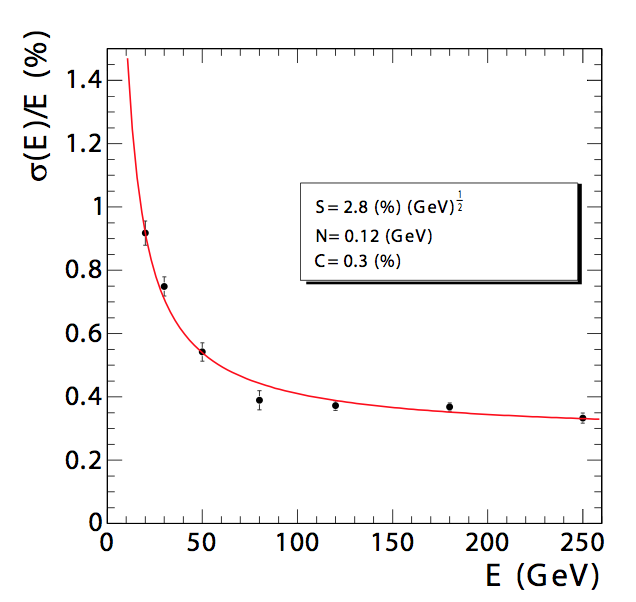
\includegraphics[width=0.85\textwidth]{plots/ecalres.png}
\caption{The CMS detector electromagnetic calorimeter energy resolution as a function of electron energy\cite{CMS_DETECTOR}.}
\label{fig:ecalres}
\end{center}
\end{figure}
